\documentclass[main.tex]{subfiles}
\begin{document}

\title{
    \textbf{Algorytmy ewolucyjne i metaheurystyki}\\
    \begin{large}
        Sprawozdanie 3
    \end{large}
}

\author{
    Górka Bartosz\\
  \texttt{127228}
  \and
  Zimniak Kajetan\\
  \texttt{127229}
}

\date{}

\maketitle

\section{Opis etapu projektu}
Celem kolejnego etapu projektu była implementacja rozszerzeń dla algorytmu \textit{Steepest}. Były to zastosowanie ruchów kandydackich oraz cache.

W projekcie wykorzystano algorytm \textit{Steepest} z bazowym przydziałem punktów do grup powstałym dzięki wykorzystaniu algorytmu naiwnego.

Jako naiwny algorytm wykorzystano algorytm przydziału punktu do grupy (bez żalu). Liczba grup pozostała bez zmian na poziomie 20.

Podobnie jak w poprzednich etapach, funkcja celu została zdefiniowana jako \textit{minimalizacja średniej odległości wszystkich par obiektów umieszczonych w ramach tej samej grupy}.

W rozdziale \ref{section:pseudokody} zaprezentowano pseudokody przygotowanych rozszerzeń algorytmu, natomiast w rozdziale\leavevmode\nobreak\ \ref{section:wyniki} wyniki działania dla 100 iteracji. Ostatni rozdział dotyczy wizualizacji najlepszych uzyskanych rozwiązań.

\section{Pseudokody rozszerzeń przeszukiwania lokalnego \textit{Steepest}}
\label{section:pseudokody}
\subsection{Ruchy kandydackie}
\begin{verbatim}
Dla każdej iteracji algorytmu Steepest wykonaj {
    Dla grupy g1 z listy grup punktów {
        Dla każdego punktu p1 w grupie g1 {
            Wyznacz najbliższy punkt p2 różny od p1 należący do grupy g2 innej niż g1
            Do listy możliwych ruchów dodaj przesunięcie punktu p1 z grupy g1 do grupy g2
        }
    }
}
\end{verbatim}

Na podstawie wyznaczonej listy możliwych przesunięć, algorytm \textit{Steepest} wybiera to, które najbardziej minimalizuje wartość funkcji celu.

\subsection{Cache}
\begin{verbatim}
Dla każdego ruchu r z listy możliwych ruchów {
    Jeżeli ruch r nie znajduje się w cache {
        Oblicz deltę zmiany funkcji celu dla ruchu r
        Zapisz deltę i ruch w pamięci cache
    }

    Z pamięci cache użyj oszacowania funkcji celu
    Jeżeli delta poprawia wartość funkcji celu {
        Zapamiętaj ruch jako dotychczas najlepszy
        Dokonaj aktualizacji aktualnej wartości funkcji celu
    }
}

Po wybraniu najlepszego z ruchów i jego wykonaniu {
    Usuń z pamięci cache przesunięcia dla grupy początkowej i docelowej, które zostały
    zmienione po wykonaniu ruchu

    Dla każdego z zapamiętanych ruchów dokonaj modyfikacji wartości
    poprzez zmianę liczby łuków i sumy ich długości.
}
\end{verbatim}

\section{Wyniki eksperymentów obliczeniowych}
\label{section:wyniki}
W tabeli \ref{table:wyniki} zaprezentowano wyniki eksperymentów obliczeniowych. Dokonano $100$ powtórzeń obliczeń. Za każdym razem algorytmy zostały uruchomione dla rozwiązań startowych zbudowanych z wykorzystaniem algorytmu naiwnego.
\begin{table}[H]
\centering
\caption{Wyniki eksperymentów obliczeniowych dla 100 iteracji}
\label{table:wyniki}
\resizebox{\textwidth}{!}{%
\begin{tabular}{|c|r|r|r|r|}
\hline
\textbf{Cecha} &                                                        \multicolumn{1}{c|}{\textbf{Naive Steepest}} & \multicolumn{1}{c|}{\textbf{Naive Steepest + Cache}} & \multicolumn{1}{c|}{\textbf{Naive Steepest + Candidates}} & \multicolumn{1}{c|}{\textbf{\begin{tabular}[c]{@{}c@{}}Naive Steepest\\with Cache + Candidates\end{tabular}}} \\ \hline
\textbf{\begin{tabular}[c]{@{}c@{}}Wartość minimalna\\funkcji celu\end{tabular}}
&   26.39
&   26.69
&   26.65
&   27.15                                                 \\ \hline
\textbf{\begin{tabular}[c]{@{}c@{}}Wartość maksymalna\\funkcji celu\end{tabular}}
&   28.67
&   32.77
&   31.25
&   34.09                                                 \\ \hline
\textbf{\begin{tabular}[c]{@{}c@{}}Wartość średnia\\funkcji celu\end{tabular}}
&   27.27
&   28.68
&   27.82
&   29.56                                                  \\ \hline
\textbf{\begin{tabular}[c]{@{}c@{}}Wartość minimalna\\czasu obliczeń {[}sec{]}\end{tabular}}
&   0.81
&   6.57
&   0.55
&   0.13                                                  \\ \hline
\textbf{\begin{tabular}[c]{@{}c@{}}Wartość maksymalna\\czasu obliczeń {[}sec{]}\end{tabular}}
&   2.32
&   40.16
&   2.05
&   2.52                                                  \\ \hline
\textbf{\begin{tabular}[c]{@{}c@{}}Wartość średnia\\czasu obliczeń {[}sec{]}\end{tabular}}
&   1.40
&   23.49
&   0.96
&   0.68                                                  \\ \hline
\end{tabular}%
}
\end{table}
Zgodnie z oczekiwaniami, zastosowanie mechanizmu łuków kandydackich pozwoliło przyspieszyć działanie algorytmu. Za zmianę czasu wykonania algorytmu musimy jednakże liczyć się z nieznacznym pogorszeniem wartości funkcji celu.

W przypadku wykorzystania mechanizmu pamięci (cache) czas realizacji jest wielokrotnie dłuższy, niż ten bez aktywnej pamięci. Jest to spowodowane aktualną funkcją celu i koniecznością aktualizacji każdego z przesunięcia jakie zostało zapamiętane. Algorytm \textit{Steepest} z liczeniem funkcji celu w formie delty (bez budowania całego rozwiązania, liczenie zmian) jest znacznie szybszy niż wielokrotne aktualizacje pamięci.

\section{Wizualizacja najlepszych rozwiązań}
Podobnie jak w poprzednim etapie projektu, również w tym zastosowano wizualizację najlepszych rozwiązań na trzy sposoby. Pierwszy z nich to zaprezentowanie samych grup punktów, bez jakichkolwiek powiązań. Drugim sposobem jest prezentacja zgodna z funkcją celu, czyli zaprezentowanie powiązań pomiędzy punktami w ramach grupy. Ostatni sposób wykorzystuje minimalne drzewo rozpinające, które w przejrzysty sposób prezentuje przydział punktów do grup.

\begin{figure}[H]
     \begin{center}
        \subfigure{
            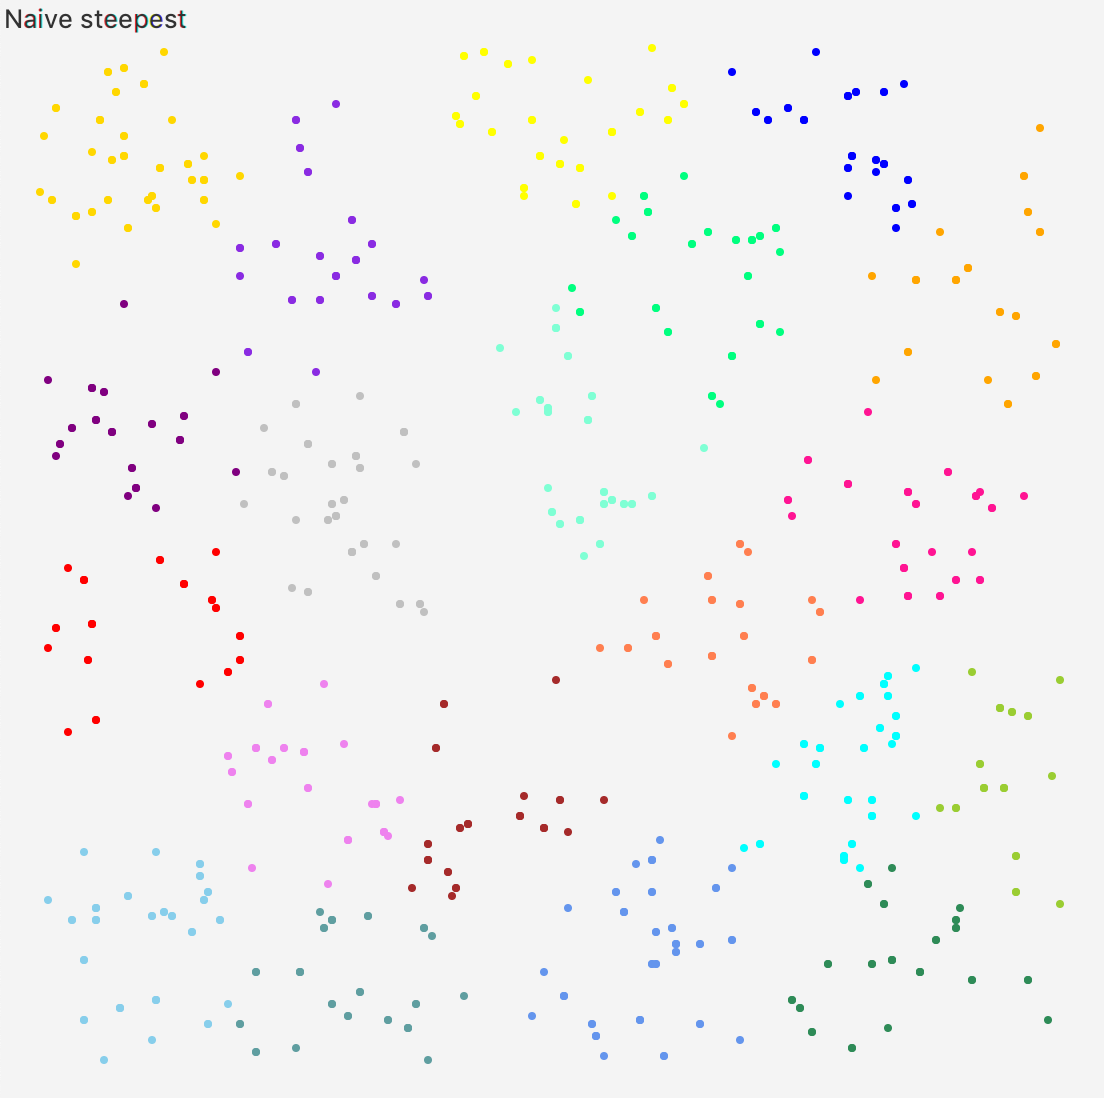
\includegraphics[width=0.45\textwidth]{sprawozdanie_3/raw_steepest.png}
        }
        \subfigure{
           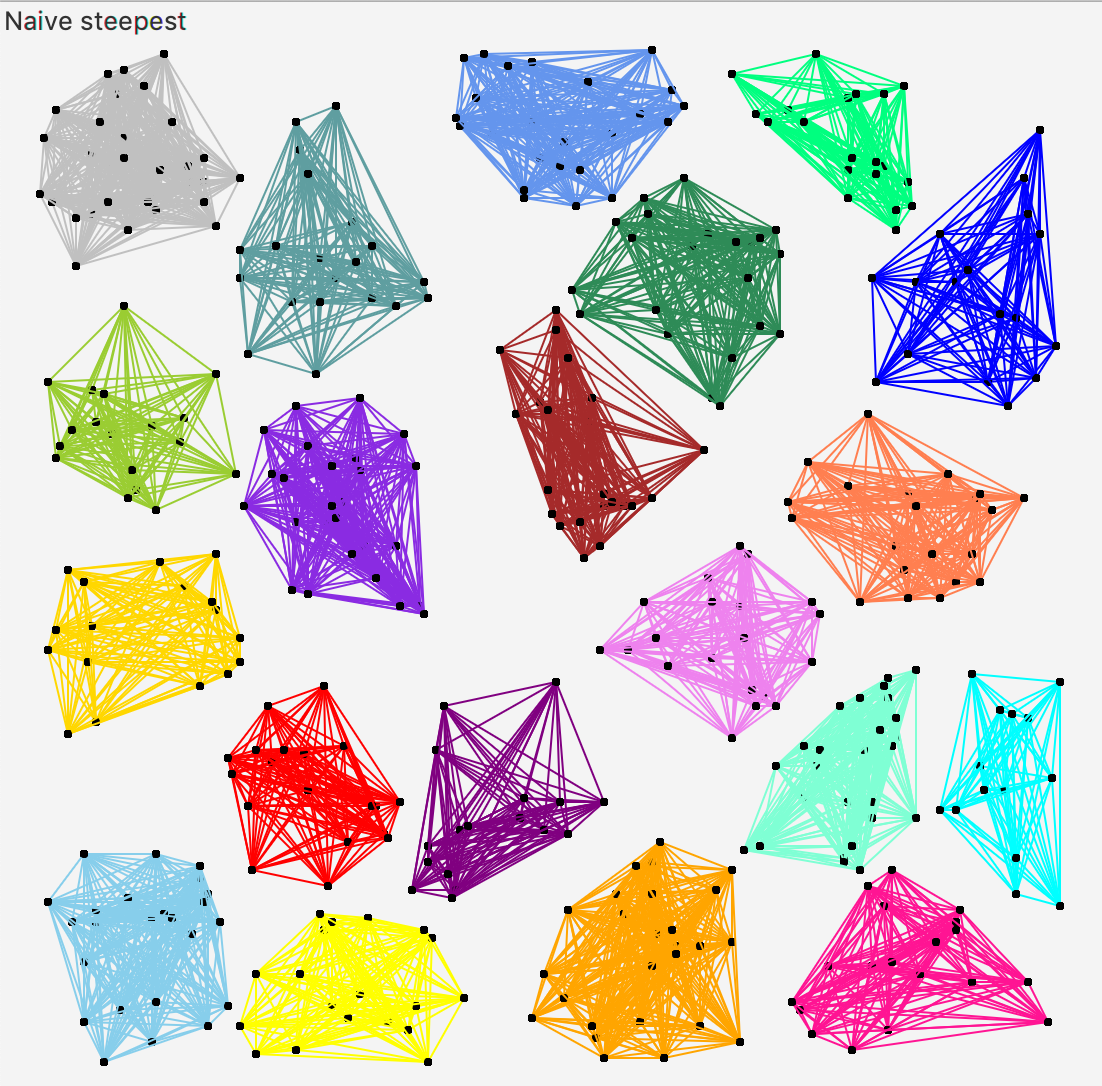
\includegraphics[width=0.45\textwidth]{sprawozdanie_3/raw_steepest_groups.png}
        }\\
        \subfigure{
            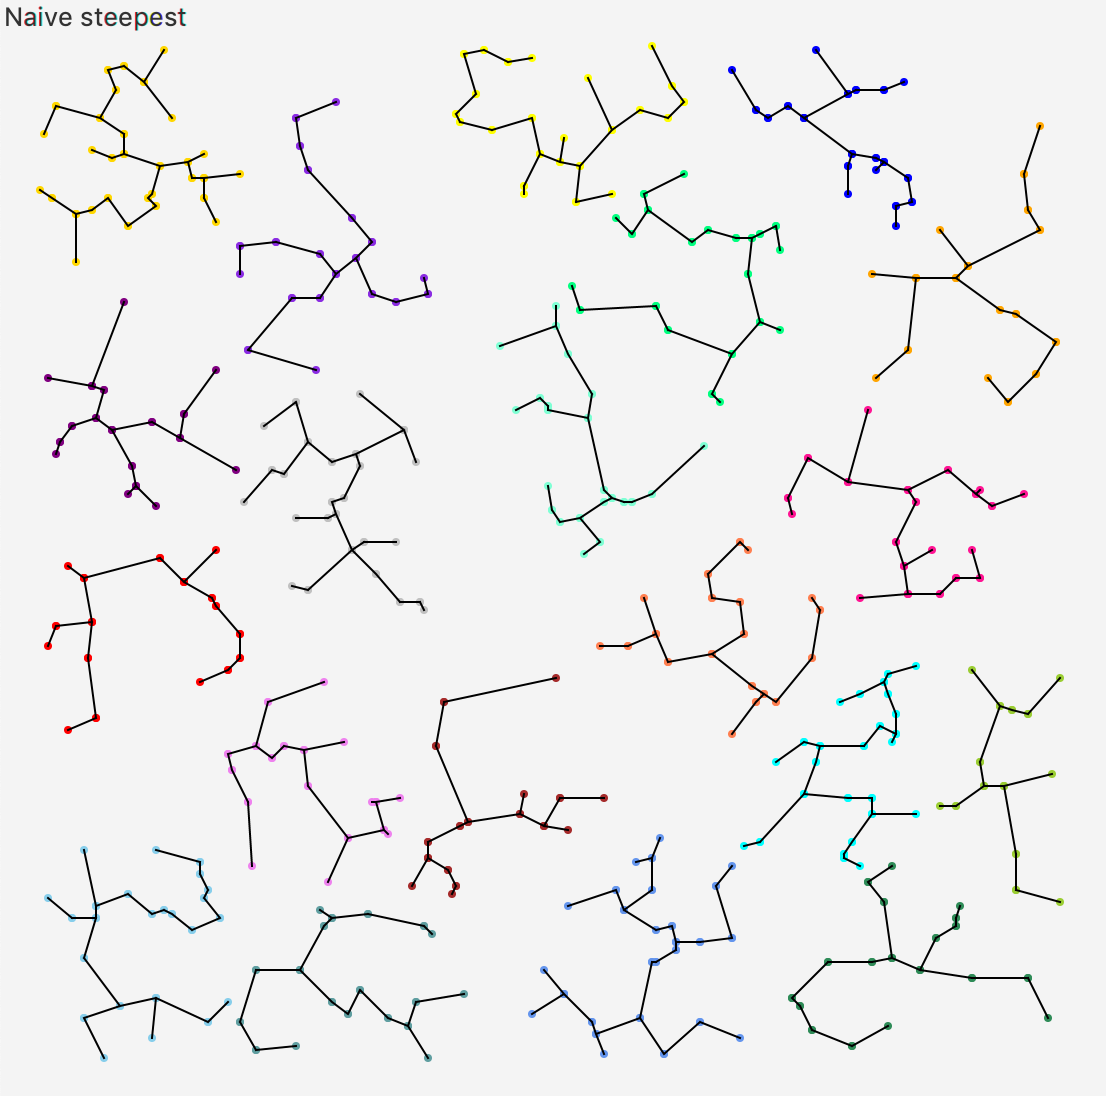
\includegraphics[width=0.45\textwidth]{sprawozdanie_3/raw_steepest_mst.png}
        }
    \end{center}
    \caption{Naive Steepst Local Search}
\end{figure}

\begin{figure}[H]
     \begin{center}
        \subfigure{
            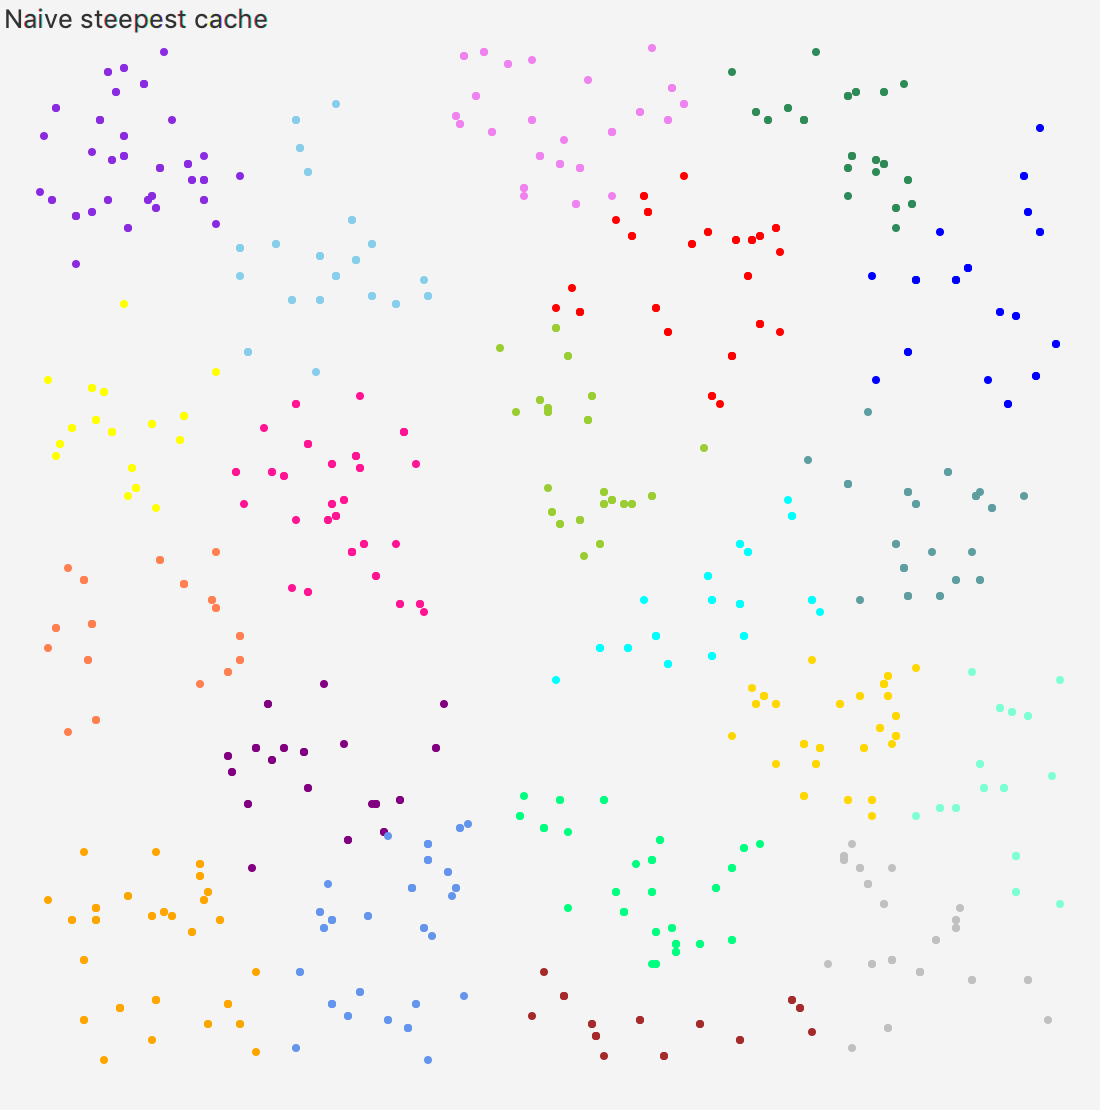
\includegraphics[width=0.45\textwidth]{sprawozdanie_3/cache.png}
        }
        \subfigure{
           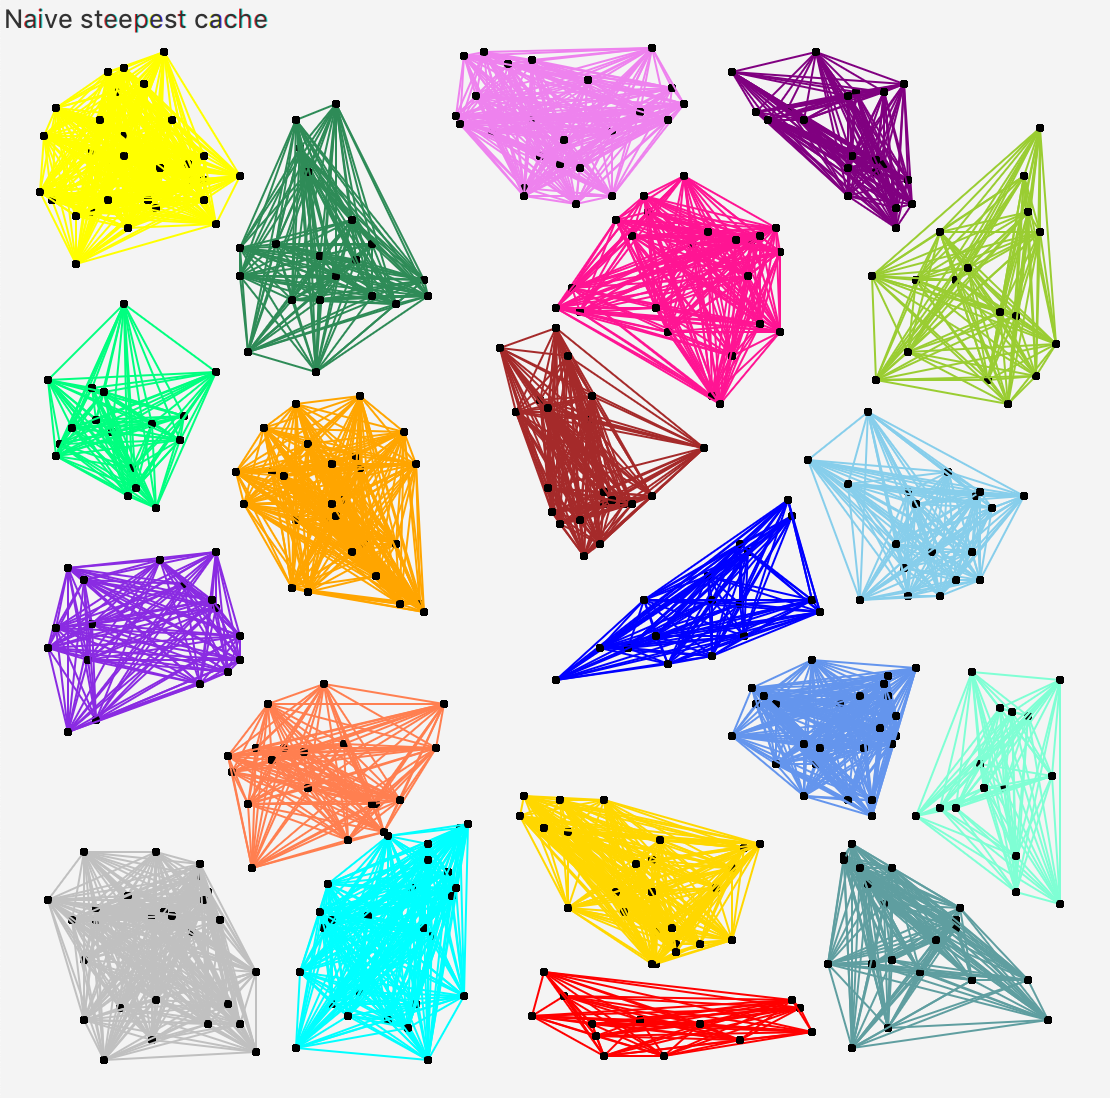
\includegraphics[width=0.45\textwidth]{sprawozdanie_3/cache_groups.png}
        }\\
        \subfigure{
            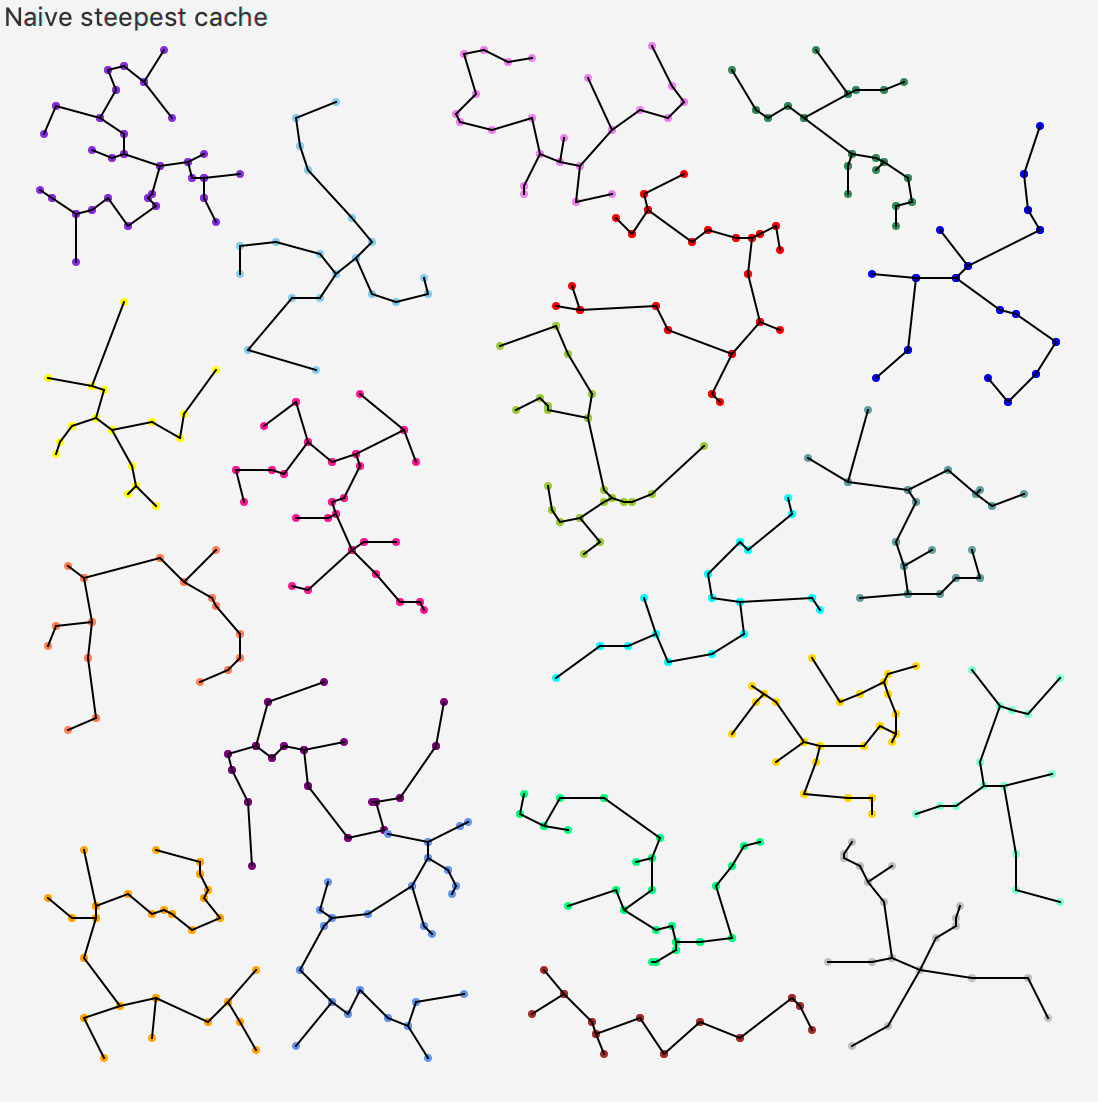
\includegraphics[width=0.45\textwidth]{sprawozdanie_3/cache_mst.png}
        }
    \end{center}
    \caption{Naive Steepst Local Search + Cache}
\end{figure}

\begin{figure}[H]
     \begin{center}
        \subfigure{
            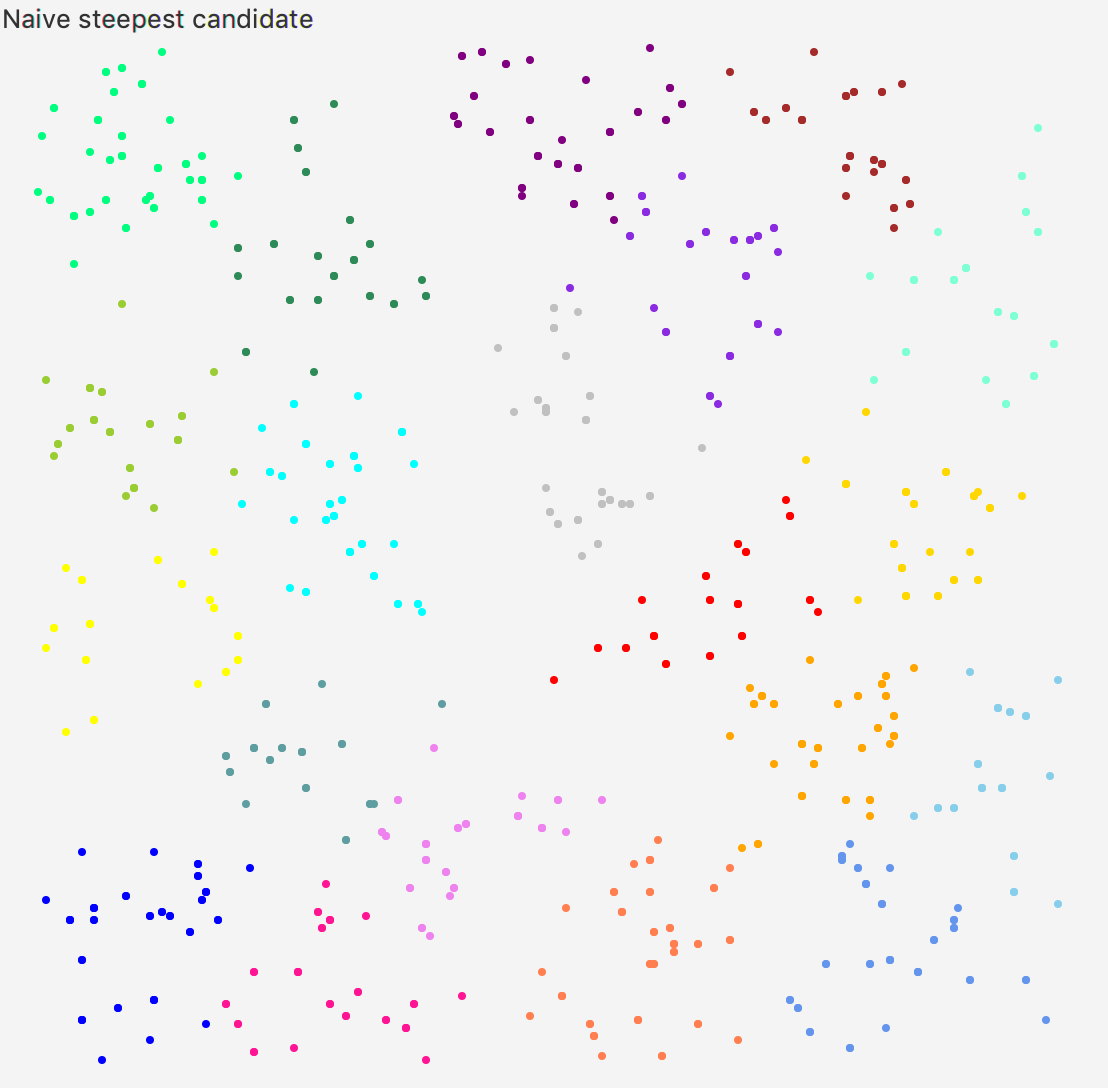
\includegraphics[width=0.45\textwidth]{sprawozdanie_3/candidate.png}
        }
        \subfigure{
           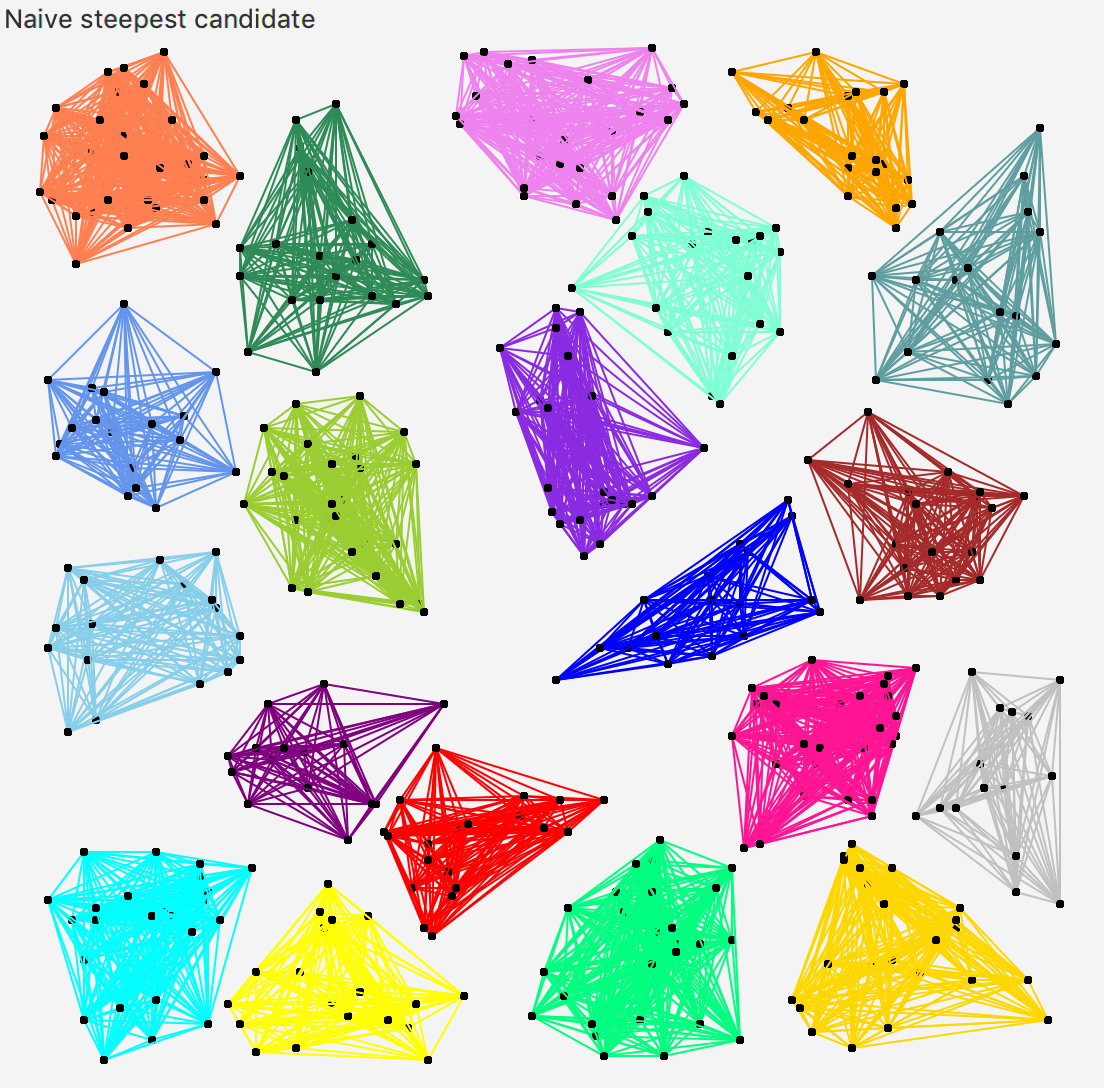
\includegraphics[width=0.45\textwidth]{sprawozdanie_3/candidate_groups.png}
        }\\
        \subfigure{
            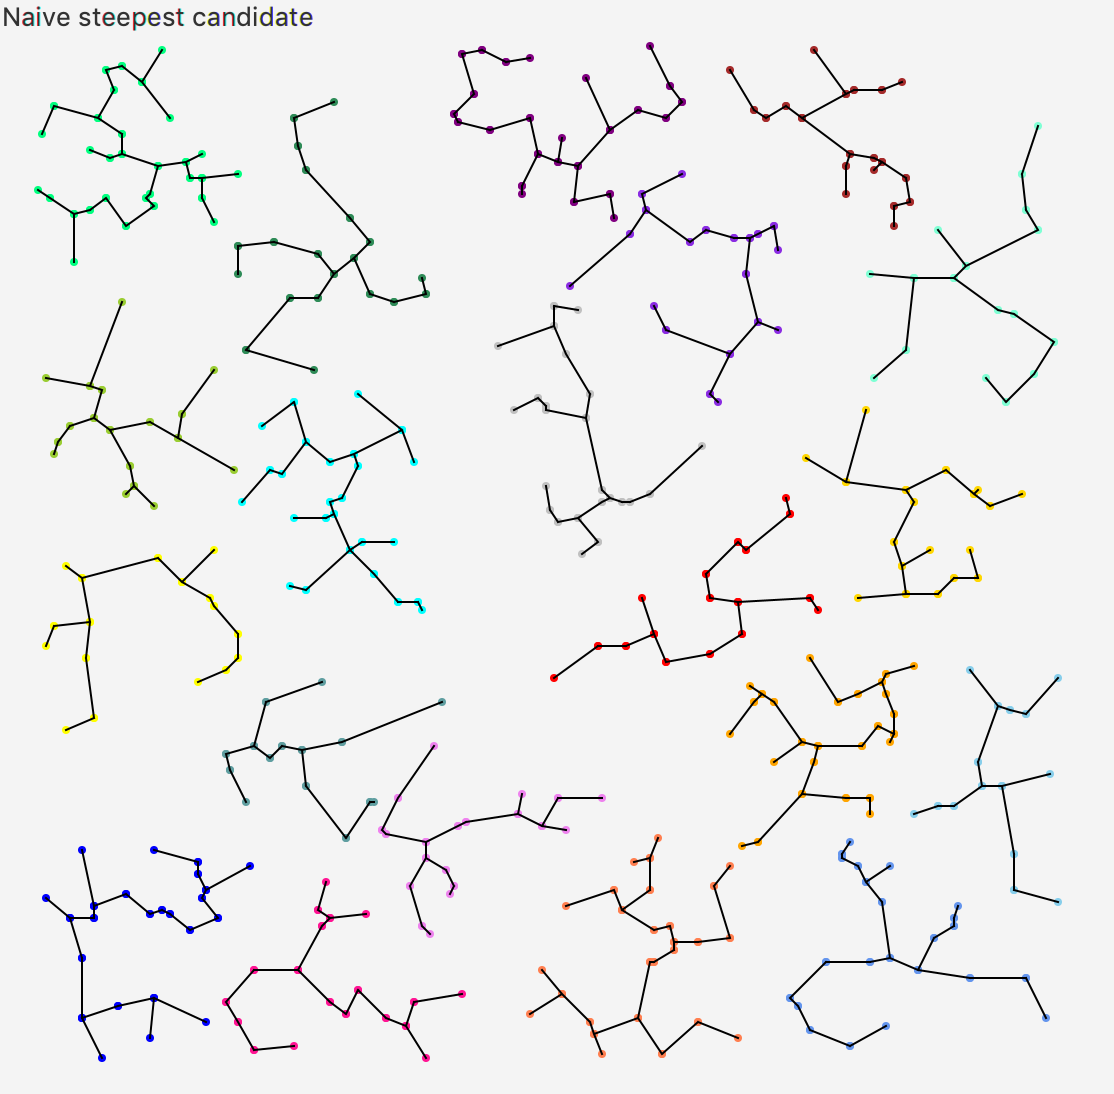
\includegraphics[width=0.45\textwidth]{sprawozdanie_3/candidate_mst.png}
        }
    \end{center}
    \caption{Naive Steepst Local Search + Candidates}
\end{figure}

\begin{figure}[H]
     \begin{center}
        \subfigure{
            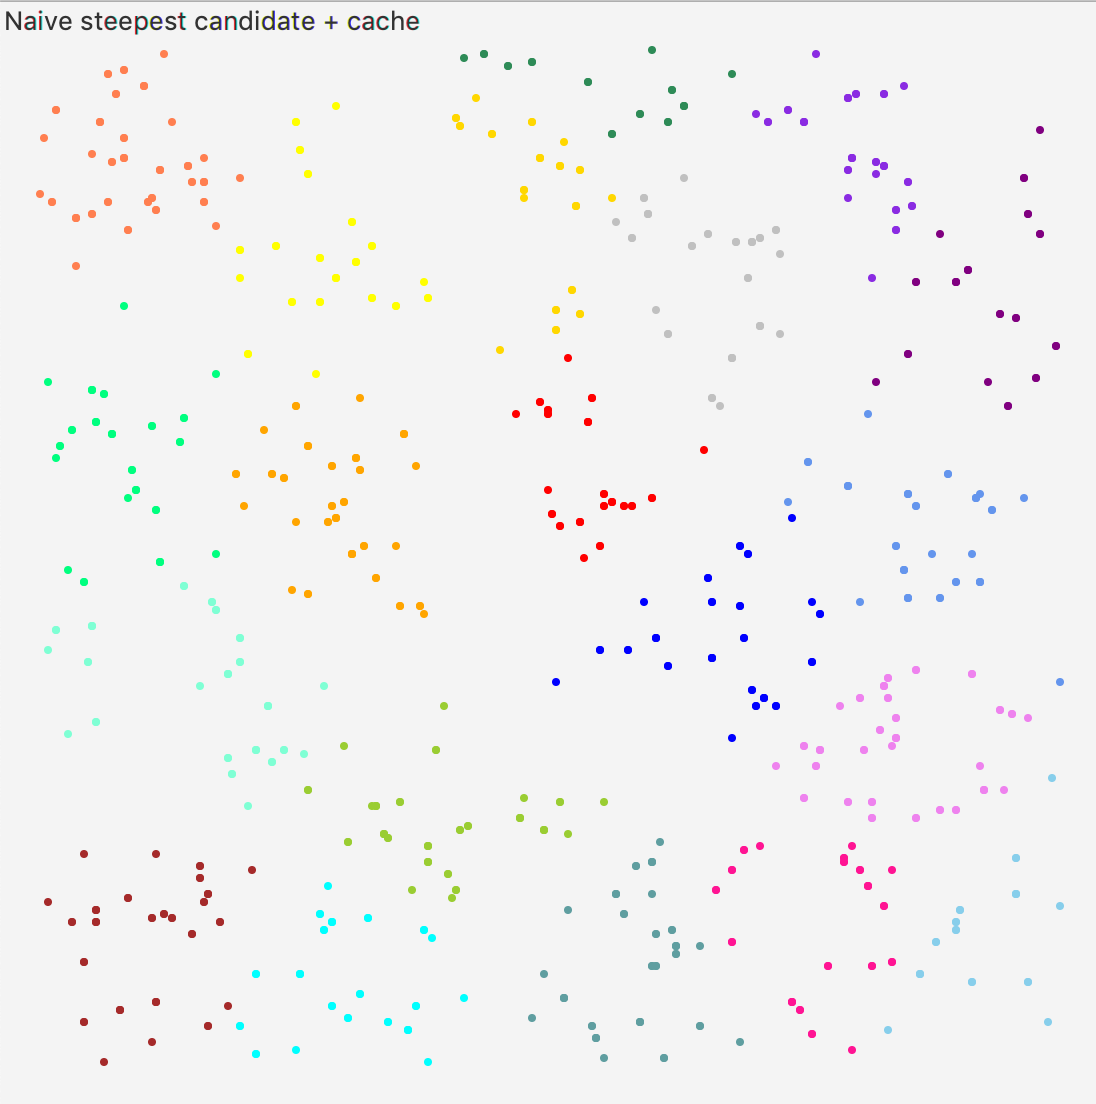
\includegraphics[width=0.45\textwidth]{sprawozdanie_3/candidates_cache.png}
        }
        \subfigure{
           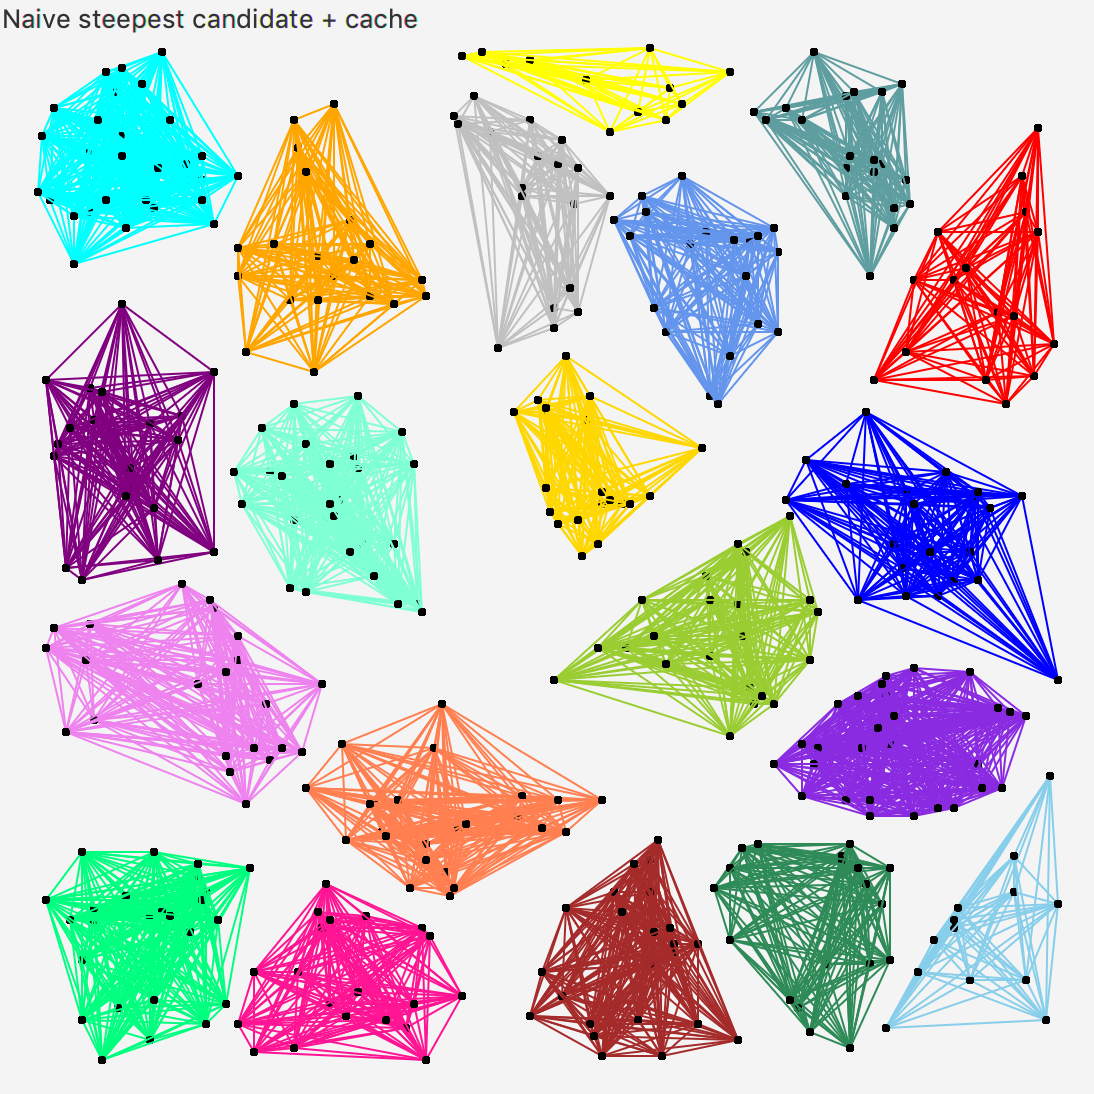
\includegraphics[width=0.45\textwidth]{sprawozdanie_3/candidates_cache_groups.png}
        }\\
        \subfigure{
            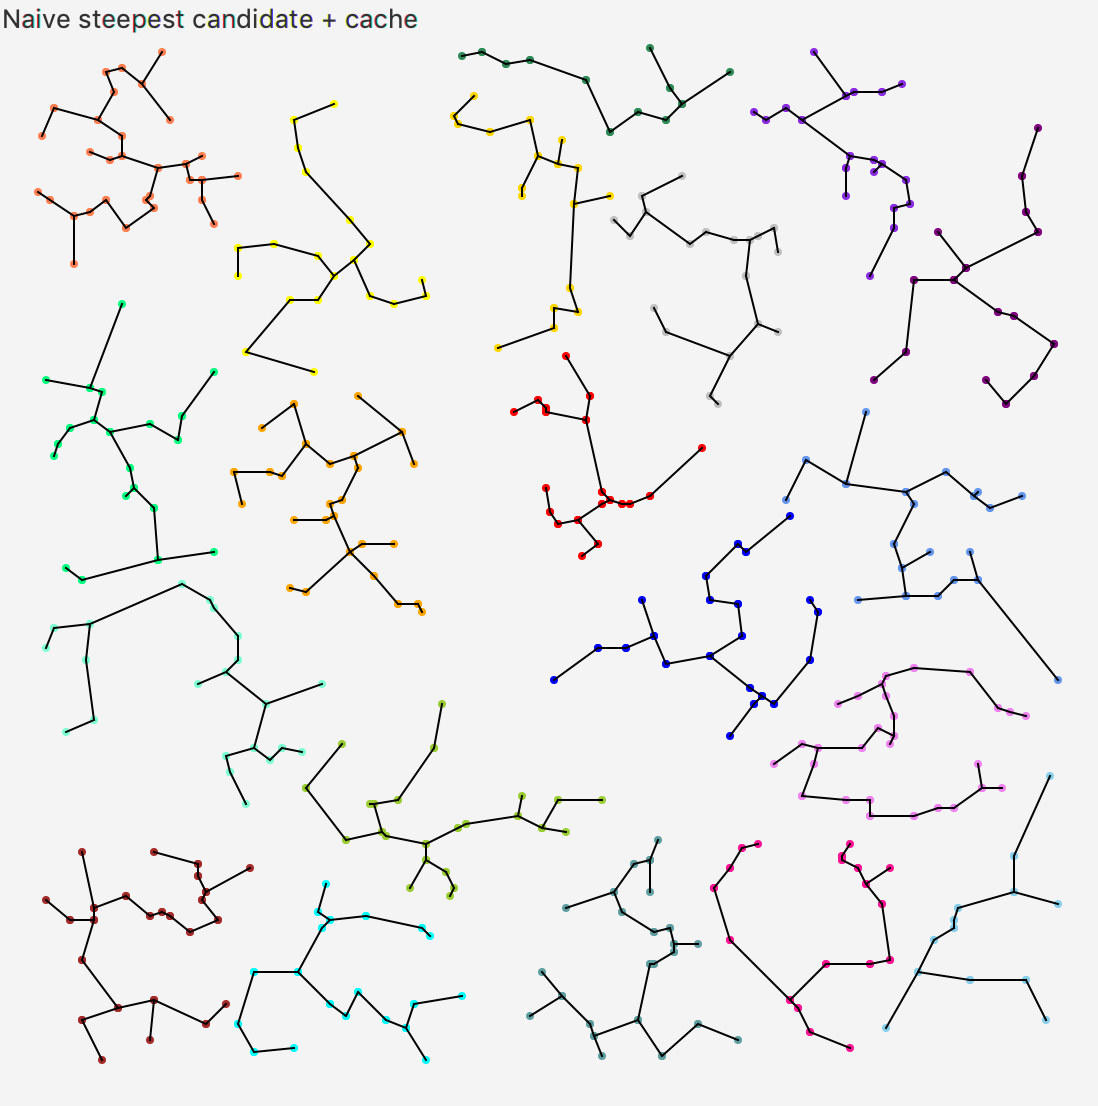
\includegraphics[width=0.45\textwidth]{sprawozdanie_3/candidates_cache_mst.png}
        }
    \end{center}
    \caption{Naive Steepst Local Search + Cache + Candidates}
\end{figure}

\end{document}